\documentclass[xcolor=dvipsnames]{beamer}

% ==== 主題 ====
\usetheme{metropolis}
\usefonttheme{professionalfonts}          % 不覆蓋你自訂的字型

% ==== 字型 ====
\usepackage{fontspec}
\usepackage{xeCJK}
\renewcommand{\familydefault}{\rmdefault} % 使用 serif 字體（重點）
\usefonttheme{professionalfonts}

% 西文字型：Times New Roman 的開源替代品
\setmainfont{TeX Gyre Termes}[
  Ligatures=TeX,
  BoldFont={* Bold},
  ItalicFont={* Italic}
]

% 中文字型（可改為思源宋體、標楷體等）
\setCJKmainfont{Noto Serif CJK TC}
\setCJKsansfont{Noto Sans CJK TC} % 有需要再用
\setCJKmonofont{Noto Sans Mono CJK TC}

% ==== 數學字型（與正文字體一致）====
\usepackage{unicode-math}
\setmathfont{TeX Gyre Termes Math}

% ==== 套件 ====
\usepackage{amsmath, amssymb}
\usepackage{graphicx}
\usepackage{hyperref}
\usepackage{minted}
\usepackage{fvextra}
\usepackage{xcolor}
\usepackage{booktabs}

% ==== 顏色設定（可選）====
\definecolor{MyBlue}{RGB}{3, 55, 105}
\setbeamercolor{structure}{fg=MyBlue}
\setbeamercolor{block title}{bg=MyBlue,fg=white}
\setbeamercolor{block body}{bg=blue!5}
\setbeamertemplate{section in toc}{%
  \inserttocsectionnumber.~\inserttocsection\par
}

\setminted{
    linenos,                % 行號
    frame=lines,            % 上下框線
    framesep=5pt,           % 程式碼與邊框距離
    numbersep=8pt,          % 行號與程式碼距離
    fontsize=\scriptsize,   % 字體大小
    breaklines,             % 自動換行
    tabsize=4,              % tab 寬度
    rulecolor=\color{black},% 框線顏色
    xleftmargin=1.5em       % 左側縮排
}

\title{Review 2 \& Time Complexity}
\author{Tai, Wei Hsuan}
\date{week 2}

\begin{document}
	\begin{frame}
		\titlepage
	\end{frame}

    \begin{frame}
        \frametitle{\href{https://drive.google.com/drive/folders/1IN7Dv6ozKHldRXJG6mI0DmjhBlwO6KWK?usp=sharing}{課程簡報}}
        \begin{figure}
            \centering
            
\includegraphics[width=0.7\textwidth]{src/qrcode.png}
        \end{figure}
    \end{frame}

    \begin{frame}
        \frametitle{Outline}
        \tableofcontents
    \end{frame}

    \section{Review}
    \begin{frame}[fragile]
        \frametitle{Basic Structure of C++ Code}
        \begin{minted}{C++}
            #include<bits/stdc++.h>
            using namespace std;

            int main(){
                // do sth
                return 0;
            }
        \end{minted}
    \end{frame}

    \begin{frame}[fragile]
        \frametitle{Array Review}
        To read $n(n\le 10^4)$ integers into an array, we can use the following code snippet:
        \begin{minted}{C++}
            int arr[10005];
            for(int i=0;i<n;++i){
                cin >>arr[i];
            }
        \end{minted}
        We often declare an array with a size slightly larger than the maximum input size to avoid out-of-bounds errors. In this case, since $n$ can be up to $10^4$, we declare the array with a size of $10005$.\\
        Though you can also utilize \texttt{int arr[n]} to declare an array, it is not recommended because it is not supported in all C++ compilers.
    \end{frame}
    \begin{frame}[fragile]
        \frametitle{Two Dimensional Array}
        The usage of two dimensional array is similar to one dimensional array, just use different indexes.
        \begin{minted}{C++}
            int arr[105][105];
            for(int i=0;i<n;++i){
                for(int j=0;j<m;++j){
                    cin >>arr[i][j];
                }
            }
        \end{minted}
    \end{frame}
    \begin{frame}
        \frametitle{More dimensional Array}
        You can also declare more dimensional array. Though it is not intuitive, it is still useful in some cases. For example, you can utilize a 5-dim array to solve a 5 unknows problem.
    \end{frame}

    \section{Time Complexity}
    \begin{frame}
        \frametitle{Basic Concept}
        Sometimes, you may get \texttt{TLE} when you submit your code. \texttt{TLE} stands for \textbf{Time Limit Exceeded}, which means your code is too slow to run within the time limit set by the online judge. To avoid getting \texttt{TLE}, you need to analyze the time complexity of your algorithm and optimize it if necessary. \\
        A computer can rouhghly execute $10^8$ operations per second. An operation can be an arithmetic operation, a comparison, or a memory access. For instance, adding two numbers, comparing two values, or accessing an element in an array are all considered operations.
    \end{frame}
    \begin{frame}
        \frametitle{What is time complexity}
        Time complexity is a way to describe how the running time of an algorithm changes as the input size increases. It is usually expressed using Big O notation, which gives an upper bound on the growth rate of the running time. For example, if an algorithm has a time complexity of $O(n)$, it means that the running time grows linearly with the input size $n$. If an algorithm has a time complexity of $O(n^2)$, it means that the running time grows quadratically with the input size $n$.
    \end{frame}

    \begin{frame}
        \begin{figure}
            \centering
            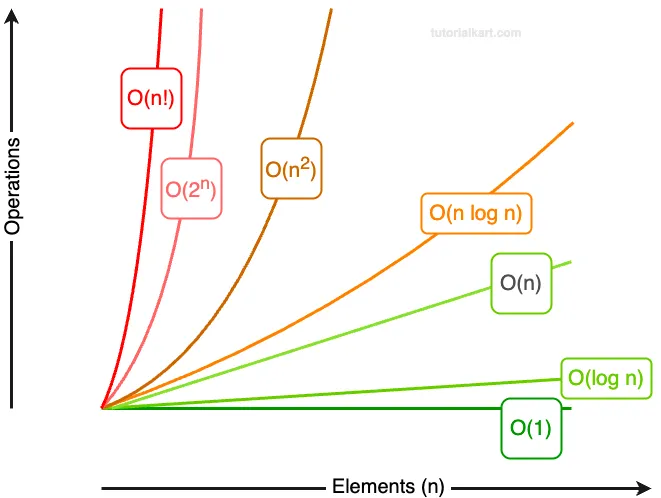
\includegraphics[width=\textwidth]{src/time_complexity.png}
        \end{figure}
        \footnotesize{Source: https://www.tutorialkart.com/algorithms/time-complexity/\#google\_vignette}
    \end{frame}

    \begin{frame}[fragile]
        \frametitle{Example}
        Consider the following code snippet:
        \begin{minted}{C++}
            for(int i=0;i<n;++i){
            }
        \end{minted}
        What is the time complexity of this code?
    \end{frame}

    \begin{frame}[fragile]
        \frametitle{Example}
        Consider the following code snippet:
        \begin{minted}{C++}
            for(int i=0;i<n;++i){
                for(int j=0;j<n;++j){
                }
            }
        \end{minted}
        What is the time complexity of this code?
    \end{frame}

    \begin{frame}[fragile]
        \frametitle{Example}
        Consider the following code snippet:
        \begin{minted}{C++}
            for(int i=0;i<n;++i){
                for(int j=0;j<i;++j){
                }
            }
        \end{minted}
        What is the time complexity of this code?
    \end{frame}

    \begin{frame}[fragile]
        \frametitle{Example}
        Consider the following code snippet:
        \begin{minted}{C++}
            for(int i=0;i<n;++i){
                for(int i=0;i<n;++i){
                }
            }
        \end{minted}
        What is the time complexity of this code?
    \end{frame}

    \begin{frame}
        \frametitle{Algorithm Choosing}
        We talked about that a computer can roughly execute $10^8$ operations per second. We should choose a proper algorithm based on the input size. For example, if the input size is $n \leq 10^5$, we can use an algorithm with a time complexity of $O(n \log n)$ or better. If the input size is $n \leq 10^3$, we can use an algorithm with a time complexity of $O(n^2)$ or better. If the input size is $n \leq 20$, we can use an algorithm with a time complexity of $O(2^n)$ or better.\\
        But the most common status is that the input size is $n \leq 5\times 10^6$, so we should always try to find an algorithm with a time c  omplexity of $O(n)$ or better.
    \end{frame}

    \begin{frame}
        \frametitle{Algorithm Analysis}
        Consider a binary search algorithm, what's the time complexity of it?
    \end{frame}

    \begin{frame}
        \frametitle{Problem Example}
        Zerojudge d563
    \end{frame}

\end{document}  